% Asset ID: AS2ForcesTikZ-006
% Source: Chapter 5/7 Forces Transcript + MechYr2 Chapter 5 Friction PDF
% Related lesson section: Worked Example 7
% Purpose: Show a particle sliding down a rough slope with friction acting up the slope.
\documentclass[tikz,border=8pt]{standalone}
\usepackage{amsmath}
\usetikzlibrary{arrows.meta, angles, quotes, decorations.pathmorphing}
\begin{document}
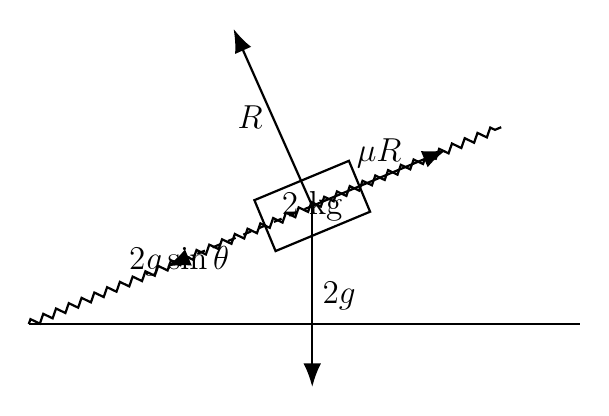
\begin{tikzpicture}[force/.style={-{Latex[length=3mm]}, thick}, comp/.style={-{Latex[length=3mm]}, thick, dashed}, label/.style={font=\large}, note/.style={font=\normalsize}]

\coordinate (A) at (0,0); \coordinate (B) at (7,0); \coordinate (C) at (6,2.5); \draw[thick] (A)--(B); \draw[thick, decorate, decoration={zigzag, segment length=5pt, amplitude=1.4pt}] (A)--(C);
\begin{scope}[shift={(3.6,1.5)}, rotate=22.6]\draw[thick] (-0.65,-0.35) rectangle (0.65,0.35); \node[label] at (0,0) {$2\text{ kg}$};\end{scope}
\coordinate (O) at (3.6,1.5); \draw[force] (O)--++(0,-2.3) node[midway,right,label] {$2g$}; \draw[force] (O)--++(-1.0,2.25) node[midway,left,label] {$R$};
\draw[force] (O)--++(1.7,0.71) node[midway,above,label] {$\mu R$}; \draw[comp] (O)--++(-1.85,-0.77) node[midway,below left,label] {$2g\sin\theta$};
\end{tikzpicture}
\end{document}
